%% basics.tex
%%
\chapter{Einführung in Projektionen}

\section{Allgemeines}

Will man einen Ausschnitt der Oberfläche einer Sphäre, beispielsweise ein Land auf dem Erdball, auf einer ebenen Oberfläche wie einem Bildschirm oder einem Blatt Papier darstellen, so muss eine Funktion aufgestellt werden, die einen dreidimensionalen Punkt (üblicherweise erfolgt die Darstellung hier durch ein Paar aus Breiten- und Längengrad) in einen zweidimensionalen Punkt umwandelt. Eine solche Funktion nennt man Projektion.

Hierbei ist zu beachten, dass mit dem Verlust einer räumlichen Dimension bei der Anwendung einer Projektion stets ein gewisser Informationsverlust beziehungsweise eine -verfälschung einhergeht. Betroffen sein können hierbei der Flächeninhalt der projizierten Struktur, die Länge einer Strecke innerhalb dieser, oder Winkel innerhalb eines Streckenverlaufs. Bewerkstelligt es eine Projektion, bei mehreren projizierten Strukturen eine der genannten Eigenschaften für alle Strukturen um einen konstanten Faktor verzerrt (üblicherweise verkleinert) wiederzugeben, wird diese Projektion flächen-/längen-/winkeltreu genannt.

\section{Kategorisierung von Projektionen}

Projektionen können in folgende Kategorien eingeteilt werden:

\paragraph{Azimutalprojektion}

Bei einer Azimutalprojektion wird die Sphäre ohne Zwischenschritte direkt auf eine Ebene projiziert.

\begin{figure}[H]
    \centering
    
    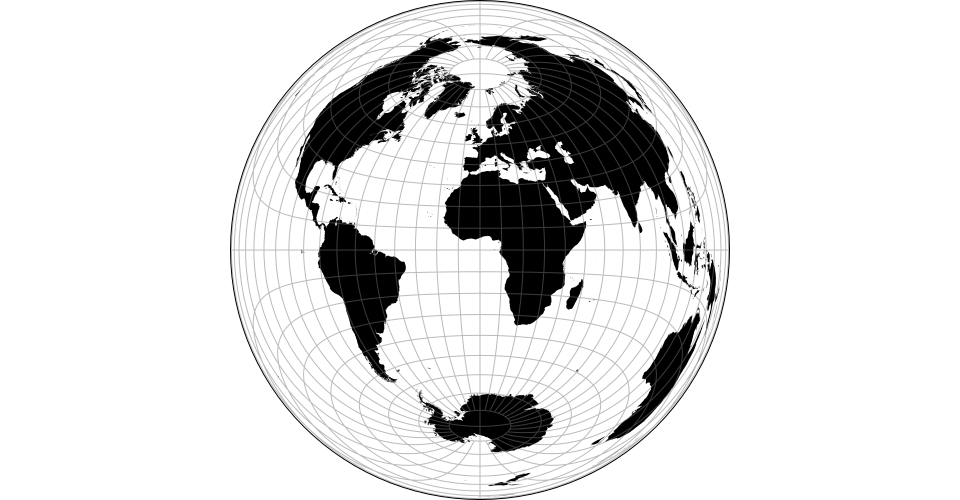
\includegraphics[width=.5\textwidth]{images/azimuthalEqualArea}
    \caption{Flächentreue Azimutalprojektion}
\end{figure}

\begin{figure}[H]
    \centering
    
    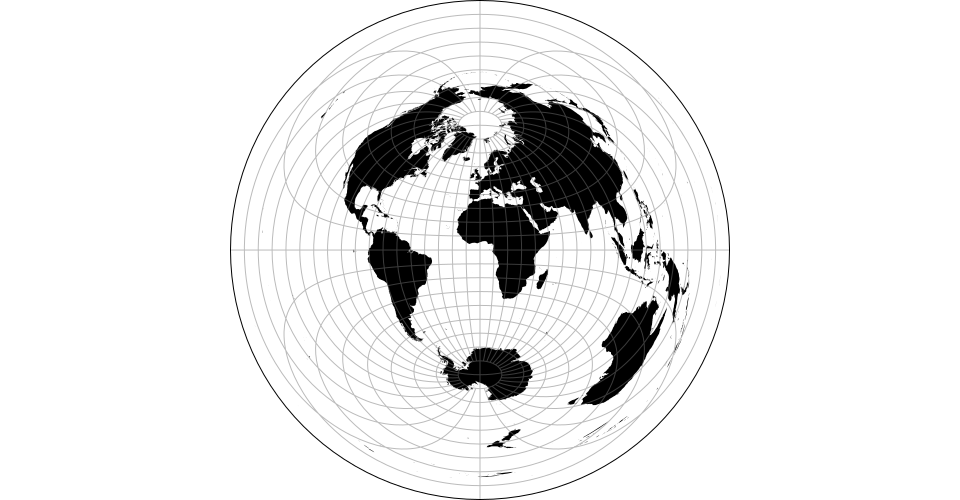
\includegraphics[width=.5\textwidth]{images/azimuthalEquidistant}
    \caption{Längentreue Azimutalprojektion}
\end{figure}

\paragraph{Konische Projektion}

Bei einer konischen Projektion wird die Sphäre zunächst auf einen Kegel projiziert. Dieser wird dann aufgeschnitten und auf eine Ebene ausgerollt.

\begin{figure}[H]
    \centering
    
    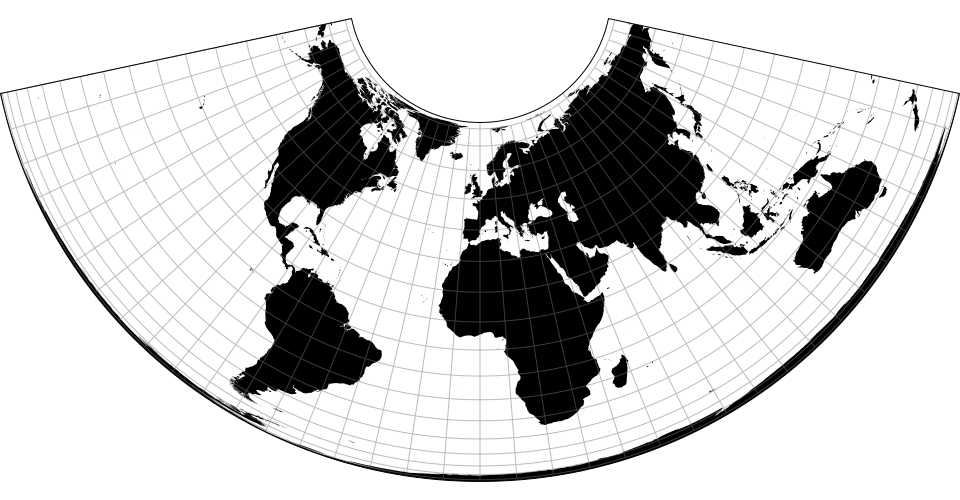
\includegraphics[width=.5\textwidth]{images/conicEqualArea}
    \caption{Flächentreue konische Projektion}
\end{figure}

\begin{figure}[H]
    \centering
    
    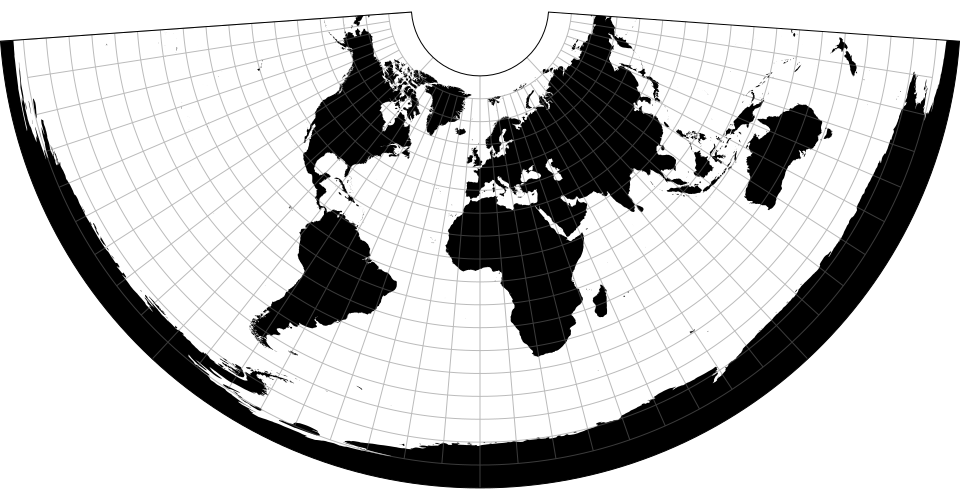
\includegraphics[width=.5\textwidth]{images/conicEquidistant}
    \caption{Längentreue konische Projektion}
\end{figure}

\paragraph{Zylindrische Projektion}

Bei einer zylindrischen Projektion wird die Sphäre zunächst auf einen Zylinder projiziert. Dieser wird dann aufgeschnitten und auf eine Ebene ausgerollt.

\begin{figure}[H]
    \centering
    
    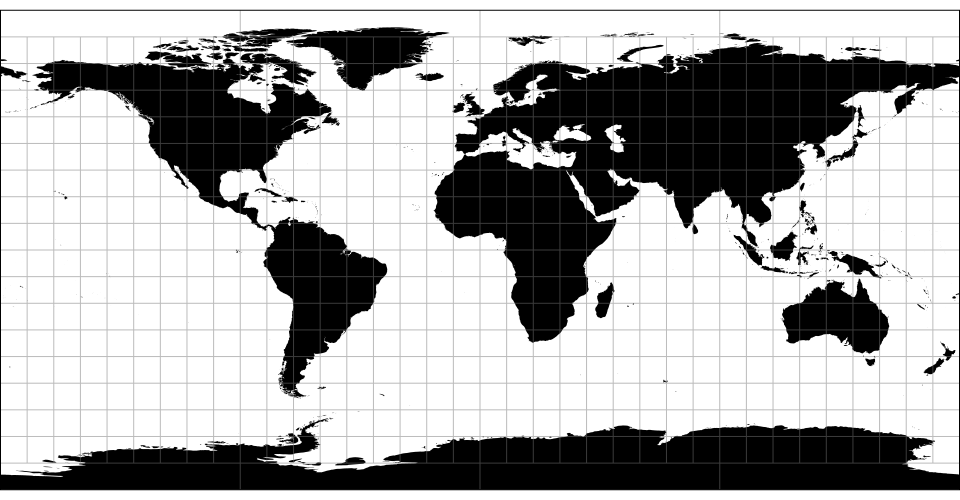
\includegraphics[width=.5\textwidth]{images/equirectangular}
    \caption{Längentreue Zylinderprojektion}
\end{figure}

\begin{figure}[H]
    \centering
    
    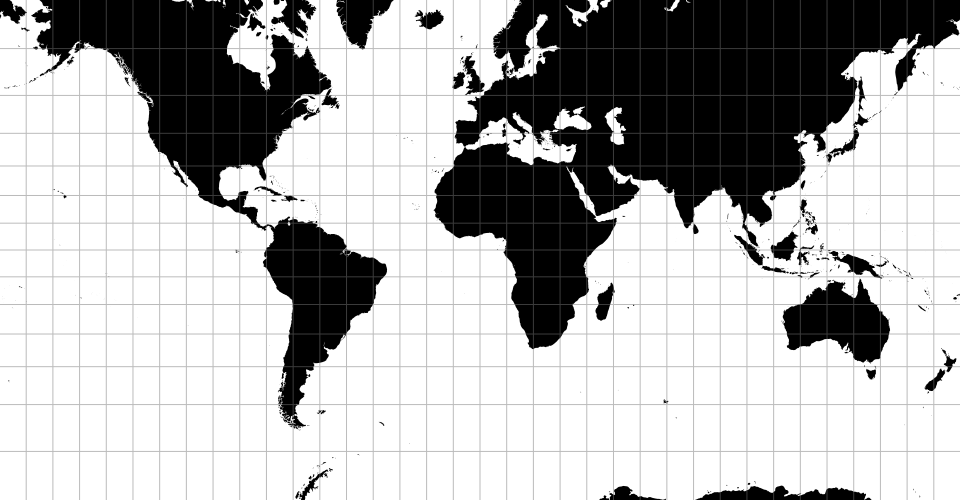
\includegraphics[width=.5\textwidth]{images/mercator}
    \caption{Winkeltreue Zylinderprojektion}
\end{figure}

\paragraph{Pseudozylindrische Projektion}

Pseudozylindrische Projektionen stellen eine Verallgemeinerung zylindrischer Projektionen dar. Breitengrade werden ebenso als parallele Linien projiziert, allerdings sind Höhengrade der konkreten Projektion entsprechend geneigt.

\begin{figure}[H]
    \centering
    
    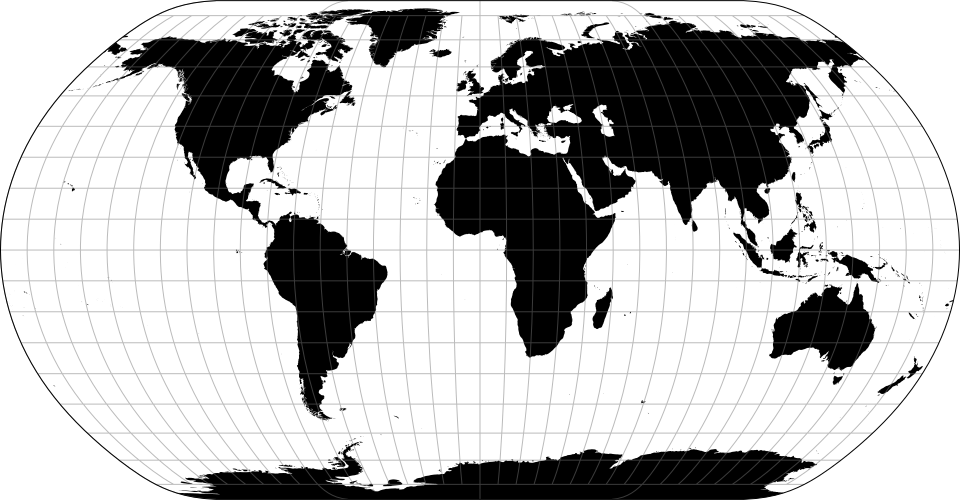
\includegraphics[width=.5\textwidth]{images/naturalEarth1}
    \caption{\glqq Natural Earth\grqq -Projektion}
\end{figure}

\paragraph{Zusammengesetzte Projektion}

Zusammengesetzte Projektionen kombinieren verschiedene der oben genannten Projektionen. Im Gegensatz zu den anderen Kategorien werden zusammengesetzte Projektionen selten für die Darstellung der gesamten Welt, sondern häufiger lediglich für Ausschnitte ebendieser genutzt.

\begin{figure}[H]
    \centering
    
    \includegraphics[width=.5\textwidth]{images/albersUSA}
    \caption{Albers-USA-Projektion}
\end{figure}

Hier wird die Albers-USA-Projektion gezeigt, die den Hauptteil der USA als konische Projektion, allerdings aus Platzgründen Alaska und Hawaii in der linken unteren Ecke um einen Faktor von etwa $0.35$ verkleinert als zylindrische Projektion darstellt.

\paragraph{Anmerkung}

Bei Betrachtung der Abbildungen fällt auf, dass keine der Kategorien Treue hinsichtlich einer Eigenschaft bedingt oder fördert, und diese lediglich der Optik dienlich sind.
